% Time-stamp: <2023-10-02 11:26:35 vladimir>
% Copyright (C) 2019-2023 Vladimir G. Ivanović
% Author: Vladimir G. Ivanović <vladimir@acm.org>
% ORCID: https://orcid.org/0000-0002-7802-7970

\chapter{Findings}\label{ch:findings}\noindent
This chapter presents data found using the approach outlined in \prettyref{ch:methods} with the goal of answering my research question: ```Has Rocketship structured itself and its finances, to earn a return to investors, focusing especially on real estate transactions, and if so, how?''

The first section presents Rocketship's corporate structure, a structure that separates Rocketship schools from Rocketship facilities. The next section, \prettyref{sec:location-and-property-info}, details what facilities Rocketship has, where those facilities are located, when they were acquired, and what real estate rights Rocketship has in those properties. Then, given Rocketship real estate, the third section characterizes the finances of Rocketship that are used to fund those properties. The penultimate section reviews what gaps, anomalies and discrepancies were found in Rocketship's financial data. The final section, \prettyref{sec:issues_equality_equity}, looks briefly at issues of fairness.

Not that Rocketship financial data is not available for all years, and starting in 2014, the data is for all of Rocketship Education, including schools in Wisconsin, Tennessee, and Washington, D.C.

\section{Rocketship's Corporate Structure}\indent%
\label{sec:RSED-corporate-structure}

Since one of the original four members of Rocketship's board of directors, Eric Resnick, ```provid[ed] a deep
understanding of financial management and real estate transactions'' \parencite{Danner2006}%p.13
, it appears that Rocketship's corporate structure was designed from the start to keep schools and their facilities separate. This structure is diagrammed in \prettyref{fig:corporate-structure} on p.\pageref{fig:corporate-structure}.

\begin{figure}[t]
  \centering\scriptsize
  \caption{\small\emph{Rocketship's Corporate Structure (Santa Clara County facilities only) Schools}}\label{fig:corporate-structure}
  \sffamily
  \begin{forest}
        for tree={grow'=east, folder, draw, align=left}
    [ \textbf{Rocketship Education}, baseline
      [ Launchpad Development Company
        [ \textit{Launchpad (LP)}, xshift=2em ]
        [ \textit{Launchpad Development One LLC (LLC1) RMS facilities}, xshift=2em ]
        [ \textit{Launchpad Development Two LLC (LLC2) RSSP facilities}, xshift=2em ]
        [ \textit{Launchpad Development Threee LLC (LLC3) RLS facilities}, xshift=2em ]
        [ \textit{Launchpad Development Four LLC (LLC4) ROMO facilities}, xshift=2em ]
        [ \textit{Launchpad Development Five LLC (LLC5) RDP facilities}, xshift=2em ]
        [ \textit{Launchpad Development Eight LLC (LLC8) RSA facilities}, xshift=2em ]
        [ \textit{Launchpad Development Ten LLC (LLC10) RSK facilities development}, xshift=2em ]
        [ \textit{Launchpad Development Eleven LLC (LLC11) RBM facilities}, xshift=2em ]
        [ \textit{Launchpad Development Twelve LLC (LLC12) RFZ facilities}, xshift=2em ]
        [ \textit{Launchpad Development Sixteen LLC (LLC16) RRS facilities}, xshift=2em ]
       ]
      [ Rocketship Support Network (RSN) ]
      [ Rocketship Mateo Sheedy Elementary (RSM) ]
      [ Rocketship Sí-Se-Puede Academy (RSSP) ]
      [ Rocketship Los Sue (RLS) ]
      [ Rocketship Mosaic Elementary (ROMO) ]
      [ Rocketship Discovery Prep (RDP) ]
      [ Rocketship Alma Academy (RSA) ]
      [ Rocketship Brilliant Minds (RBM) ]
      [ Rocketship Spark Academy (RSK) ]
      [ Rocketship Fuerza (RFZ) ]
      [ Rocketship Rising Stars (RRS) ]
    ]
    \end{forest}
  \end{figure}

  The parent corporation, Rocketship Education, Inc. (RSED), a 501(3)(c) public benefit corporation, was formed in California on February 16, 2006. RSED owns all the Rocketship schools and Launchpad Development Company, a 509(a)(3) nonprofit public benefit corporation.\footnote{A 509(a)(3) corporation is a ``charity that carries out its exempt purposes by supporting other exempt organizations, usually other public charities'' and ``has a relationship with its supported organization sufficient to ensure that the supported organization is effectively supervising or paying particular attention to the operations of the supporting organization.'' \parencite[accessed 29 Sep 2023]{IRS2023}}  Launchpad Development Company owns one LLC for each school's facility, generally named ``Launchpad Development <number> LLC''. In addition, Rocketship has two functional divisions:
  \begin{itemize}
    \item Rocketship Support Network (RSN) which provides resources for management, back-office support, and organizational strategy to Rocketship schools
    \item Launchpad (LP) which provides investment and asset management, and administrative services to Launchpad LLCs
  \end{itemize}

  This separation between the operation of schools from the funding of their facilities raises the question of why Rocketship has chosen this structure. Some possibilities are:
  \begin{itemize}
    \item The owners of a school's facilities are not schools and thus are not directly subject to California's Education Code.
    \item Facility owners are somewhat insulated from legal action against schools.
    \item RSED can charge schools management and facility fees that might not be allowed for schools themselves.
    \item When a charter school closes, the real estate assets (land + buildings + improvements) are not owned by the charter school, but by a separate entity (Launchpad Development One/Two/Three/\ldots) which is owned by another entity (Launchpad Development Company) that itself is owned by yet another entity (Rocketship Education). Since Launchpad Development owns other properties, it is unlikely to close if one of its schools close, thereby retaining the property as an asset.
  \end{itemize}
  
%%%%%%%%%%%%%%%%%%%%%%%%%%%%%%%%%%%%%%%%%%%%%%%%%%%%%%%%%%%%%%%%%%%%%%%%%%%%%%% 
%%% Rocketship Properties
%%%%%%%%%%%%%%%%%%%%%%%%%%%%%%%%%%%%%%%%%%%%%%%%%%%%%%%%%%%%%%%%%%%%%%%%%%%%%%%
  \section{Rocketship Locations and Property Information}\indent%
  \label{sec:location-and-property-info}
  \begin{table}[hbt]
    \caption[Rocketship Property Information]{\textit{Rocketship Property Information}}\label{tab:locations}\SingleSpacing%
    \begin{tabular}{lll}
      \toprule
      School          & Address                               & Property Information \\
      \midrule
      Mateo Sheedy    & 788 Locust St., San José, CA 95110    & \prettyref{sec:mateo-sheedy-info} \\
      Sí Se Puede     & 2249 Dobern Ave, San José, CA 95116   & \prettyref{sec:sí-se-puede-info} \\
      Los Sueños      & 331 S. 34th St, San José, CA 95116    & \prettyref{sec:los-suenos-info} \\
      Discovery Prep  & 370 Wooster Ave, San José, CA 95116   & \prettyref{sec:discover-prep-info} \\
      Mosaic          & 950 Owsley Ave, San José, CA 95122    & \prettyref{sec:mosaic-info} \\
      Brilliant Minds & 2960 Story Rd, San José, CA 95127     & \prettyref{sec:brilliant-minds-info} \\
      Alma Academy    & 198 West Alma Ave, San José, CA 95110 & \prettyref{sec:alma-academy-info} \\
      Spark Academy   & 683 Sylvandale Ave San José, CA 95111 & \prettyref{sec:spark-academy-info} \\
      Fuerza          & 70 S. Jackson Ave, San José, CA 95116 & \prettyref{sec:fuerza-info} \\
      Rising Stars    & 3173 Senter Road, San José, CA 95111  & \prettyref{sec:rising-stars-info} \\
      \bottomrule
    \end{tabular}
  \end{table}

  Details of the ownership of Rocketship schools listed in \prettyref{tab:locations} are in \prettyref{ch:rocketship-property-info} on p.\pageref{ch:rocketship-property-info}.

\section{Rocketship's Finances}\indent
\label{sec:rocketship_finances}

  Financing charter schools in California is more complicated than the financing of traditional public schools because charters need to obtain facilities, often independently from the public school district in which they are located.
\prettyref{tab:charter-school-financing-options} on p.\pageref{tab:charter-school-financing-options} describes what facilities financing options a charter school has compared to a traditional public school. Note that ending up with facilities that satisfy a school's needs may require the purchase of land, the construction of new facilities, or the modification of existing facilities in addition to operating those facilities. Each of these alternatives have different potential financing options.

\subsection{Charter School Financing Options}\indent\label{sec:charter-school-financing-options}

\begin{table}[hbt]
  \caption[Charter School Financing Options]{\textit{Charter School Financing Options}}\label{tab:charter-school-financing-options}%
  \SingleSpacing%
  \begin{tabular}{lccl}
    \toprule
    \textbf{Type}        & \multicolumn{2}{c}{\textbf{Available to}}  & \textbf{Notes}\\
                         & \textbf{TSPs} & \textbf{Charters}          & \\
    \midrule
    \multicolumn{4}{l}\textit{{State funding}} \\
    \midrule
    LCFF                 & Yes  & Yes                        & State minimum guarantee: ADA + adjustments\\ 
    Local property tax   & Yes  & Yes                        & Reduces LCFF amount\\
    Categorical programs & Yes  & Yes                        & \multirow[t]{2}{3in}{All state funding outside of LCFF is\\
                                                               categorical. Some federal programs exist.} \\
    \\
    \midrule
    \multicolumn{4}{l}{\textit{Local funding}}\\
    \midrule
    Local parcel tax     & Yes  & No                         & Established by district election\\
    Bonds                & Yes  & Yes                        & \multirow[t]{2}{3in}{TSPs: district election; \\
                                                               Charters: private only}\\
    \\
    Construction loans   & Yes  & Yes                        & \multirow[t]{3}{3in}{Typically bonds, with widely varying \\
                                                             terms, but also from the general fund.\\
                                                             Charters: private placement only}\\
    \\\\
    \midrule
    \multicolumn{4}{l}{\textit{Federal, state, or private funding}}\\
    \midrule
    Private grants       & Yes & Yes                         & Much more common with charters\\
    COVID-19 PPP loans   & No  & Yes                         & Paycheck Protection Program loan \equiv  grant\\
    Venture fund loans   & No  & Yes                         & Often using New Market Tax Credit program\\
    Rent subsidies       & No  & Yes                         & SB740\\
    \bottomrule
  \end{tabular}
\end{table}

The first three sources of financing listed above are considered ordinary revenue and are available to both public schools and to charter schools, although the amounts and timing of the distributions vary. The remainder 

\begin{itemize}
  \item \textbf{LCFF} A charter's home district passes through an amount based on a charter's demographics and ADA (Average Daily Attendance). All schools have the same base grant adjusted for grade spans. If a school, charter or public, has students who are eligible for free or reduced price meals (FRPM), or are English Learners (EL), or are foster youth, the school receives a supplemental grant of 20\% of its adjusted base grant for each such student. If the qualifying population of students exceeds 55\% of the total, a school receives 65\% of the adjusted base grant for every student above the 55\% threshold.

  Since all Rocketship schools have at least 55\% of their students , the school qualifies for a LCFF concentration grant in addition to a LCFF supplemental grant. Each qualifying student over the 55\% threshold is entitled to an additional 65\% of the LCFF base grant. Each qualifying student is entitled to an additional 20\% over the base LCFF grant.\\
  \item \textbf{Property tax} In California, all commercial or private properties are taxed. School districts receive 40\% of this property tax which replaces am equal portion of LCFF revenue. (If a district's property tax revenue exceeds what they would have gotten in LCFF funding, they receive no LCFF funding. These districts are called \textit{community-funded districts}, previously known – confusingly – as \textit{basic aid districts}.)
  \item \textbf{Parcel tax} Traditional public school district may assess a non-\textit{ad valorem} tax, usually a per parcel tax\footnote{A 2023 court decision allowed a tax based on square footage.} if voters approve. Charter schools do not have taxing authority, so they may not assess parcel taxes. Public school districts may agree to share some portion of their parcel tax revenue with charter schools within their boundaries.
  \item \textbf{Bonds} Bonds, as far as educational institutions are concerned, come in just a few forms:
  \begin{itemize}
    \item General Obligation (GO) Bonds
    GO bonds are backed by the full faith and credit of the issuer, here a school.

    Unlike public school districts that can pass a bond measure based on the value of the entire district's assessed property, charter schools have either no real property (if they are leasing) or a very small amount (if they own their facilities), so even if they were allowed to put a bond measure to the voters, the GO debt limit of 1¼\% of their facility's assessed value would provide very limited funds. For example, an \$80M valuation would be required to be able to issue a \$1M bond. 

    \item Tax and Revenue Anticipation Notes (TRANs) and Revenue Anticipation Notes (RANs)
    Revenue anticipation notes are backed by specific forms of revenue. 
    \item Conduit Revenue Bonds
    Conduit bonds are issued by and are an obligation of a government agency (the conduit) that is neither the borrower nor the purchaser. The government agency is merely a conduit between a borrower and the purchaser(s) of the bond. The conduit borrower's payments to the conduit are sized to meet the payments needed to repay the debt.
  \end{itemize}

  A complete discussion of governmental debt in California can be found in \textcite{CDIAC2023}.
  
  \item \textbf{Construction loans}  Construction loans\\
  \item \textbf{COVID-19 PPP} loans COVID-19 PPP loans\\
  \item \textbf{Venture fund loans} Venture fund loans\\
  \item \textbf{Private grants} Private grants\\
  \item \textbf{Rent subsidies} Rent subsidies\\
\end{itemize}

\subsection{Rocketship Financial Documents}\label{sec:rocketship-financial-docs}\indent

% In 2012, the Bronx Charter School for Excellence (BCSE) felt the need to purchase the facilities it was leasing. It considered
% \begin{itemize}
%   \item New Markets Tax Credits, a federal program
%   \item Local Initiatives Support Corporation (LISC), a Ford Foundation program
%   \item Civic Builders, a non-profit real estate developer and lender
%   \item the Canyon-Agassi Charter School Facilities Fund, 
%   \item direct bank loans
%   \item tax-exempt bond markets
% \end{itemize}\parencite{Clark-Herrera.etal2013}

Every year, as required by law, Rocketship issues an independently audited financial statement for the preceding school year. Rocketship, rather than issuing a separate financial statement for each of its affiliates, consolidates them into a single document, typically titled \emph{Rocketship Education, Inc. and Its Affiliates Consolidated Financial Statements and Supplementary Information Year Ended June 30, xxxx}. Four annual financial statements are reported:

\begin{itemize}
  \item Financial Position, which corresponds to a business's balance sheet\\
  \item Activities, which corresponds to a business's income statement\\
  \item Cash Flows, which corresponds to a business's cash flow statement\\
  \item Functional Expenses, which has no corresponding business statement\\
\end{itemize}

Each annual financial statement, starting with the YE 2011, includes a disclaimer such as, ``All significant inter-company accounts and transactions within RSED and its schools have been eliminated in the consolidating financial statements.'' Although this may be standard accounting practice, it does make getting a complete picture of Rocketship's finances harder because some transactions effectively disappear from the consolidated statements. These transactions are still visible in other reports.

The four different financial statements for the years 2010–2022\footnote{The years ending 2008 (2007–2008) and 2009 (2008-2009) have not been included in some summaries because they were different from all the other years. The year 2009 included 2008, and 2008 was restated in 2022.} have been collected and the data summarized. These summaries appear in \prettyref{tab:consolidated_financial_position}, \prettyref{tab:consolidated_activities}, \prettyref{tab:consolidated_cash_flows}, and \prettyref{tab:consolidated_functional_expenses}, and online in this dissertation's \textit{Data Dashboard}, a Google spreadsheet.%
\footnote{\url{https://docs.google.com/spreadsheets/d/1c4akEKFj9bmVfLFQwi7ewMifSjRbrw5xpjh_UjO4oYY/edit?usp=sharing}}

Rocketship's net assets from 2010 to 2022 have always been positive as seen in the following table, although they have varied considerably from year to year.
\begin{table}[ht]\caption{Net Assets and Annual Change, 2010–2022}\label{tab:net_assets_annual_change}
  \begin{tabular}{lll}
    \toprule
    \textbf{Year} & \textbf{Net Assets} & \textbf{Annual Increase}\\
    \midrule
    2010 &   \$2,218,964	&            \\
    2011 &   \$9,212,140	&   315.16\% \\
    2012 &  \$11,933,099	&    29.54\% \\
    2013 &  \$15,881,210	&    33.09\% \\ 
    2014 &  \$13,356,528	&   -15.90\% \\
    2015 &  \$10,562,747	&   -20.92\% \\
    2016 &  \$16,931,464	&    60.29\% \\
    2017 &  \$17,536,163	&     3.57\% \\
    2018 &  \$20,883,606	&    19.09\% \\
    2019 &  \$24,084,572        &    10.12\% \\
    2020 &  \$24,617,294        &     2.21\% \\
    2021 &  \$38,231,318	&    55.30\% \\ 
    2022 &  \$33,442,645        &   -12.53\% \\
    \bottomrule
  \end{tabular}
\end{table}

% \begin{figure}[ht]
%   \centering
%   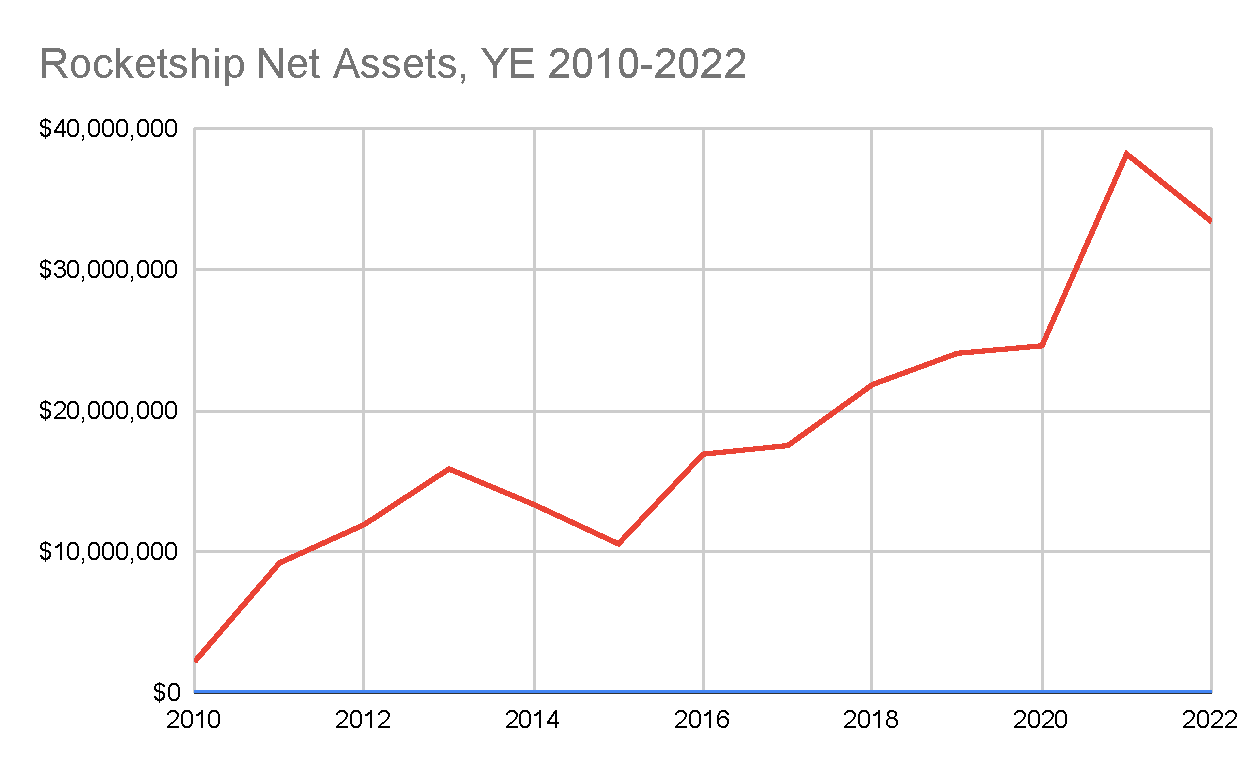
\includegraphics[width=\textwidth,keepaspectratio]{Net_Assets}%
%   \caption{Rocketship Net Assets, YE 2010-2022}%
%   \label{fig:net_assets}
% \end{figure}

% \begin{figure}[b]
%   \centering
%   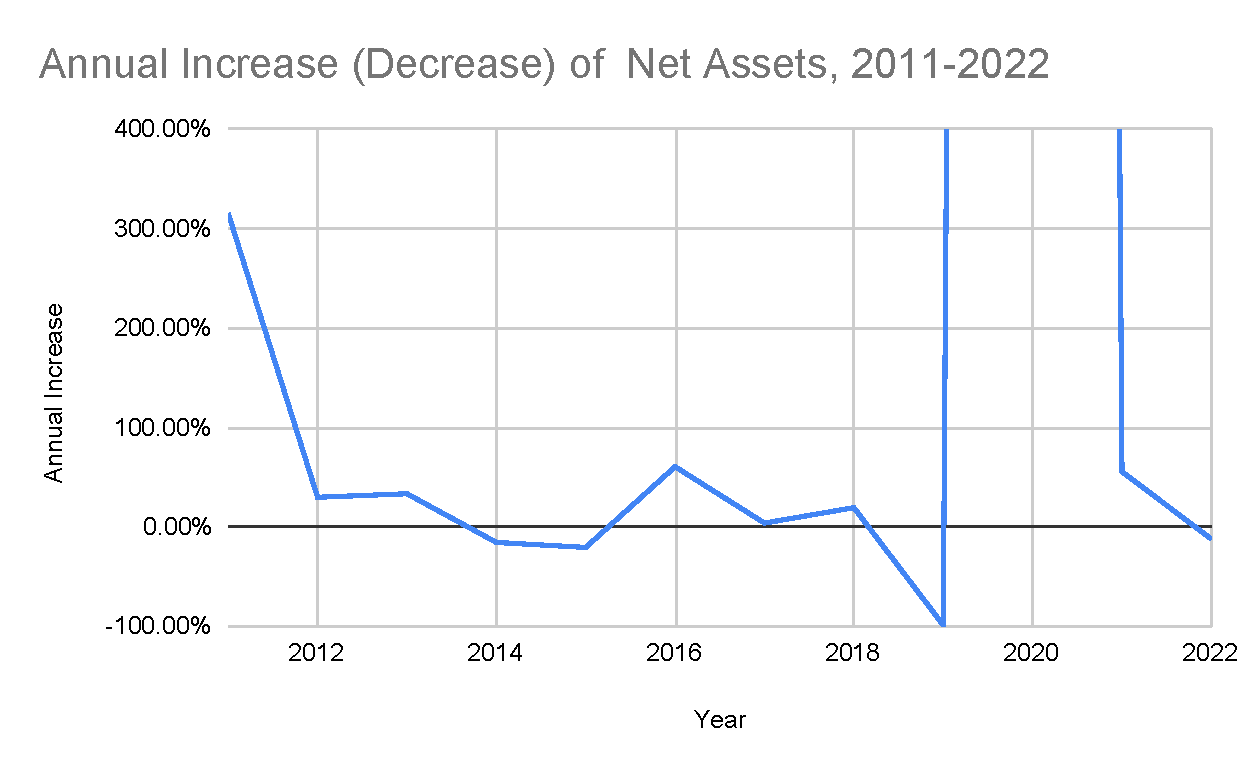
\includegraphics[width=\textwidth,keepaspectratio]{Annual_Increase_Net_Assets_2011-2022}%
%   \caption{Annual Increase in Net Assets, 2011-2022}%
%   \label{fig:annual_net_asset_increases}
% \end{figure}

\subsection{Debt}\indent%
\label{sec:debt}

Rocketship has borrowed over 50 times since its founding in 2006\footnote{Full details of Rocketship's borrowings are in this dissertation's Google spreadsheet (see the previous footnote) in the tab \textit{Dashboard} starting on lines 10–63.} 
and their annual, consolidated financial statements provide debt summaries starting in 2012. The totals are shown in \prettyref{tab:total_debt} below.

The annual increase (or decrease) in debt year over year is shown in \prettyref{tab:total_debt} One can immediately observer that the changes in debt year-over-year are quite pronounced. They range from a low of 86\% to a high of 155\% with an average of just over 100\% per year.
  
\begin{table}[ht]\caption{Total Debt, 2012-2022}\label{tab:total_debt}
  \begin{tabular}{lll}
    \toprule
    \textbf{Year} & \textbf{Total Debt} & \textbf{Annual Increase}\\
    \midrule
    2012 &  \$47,046,048 & \\
    2013 &  \$57,078,166 & 121.32\% \\
    2014 &  \$88,383,082 & 154.85\% \\
    2015 &  \$75,904,098 &  85.88\% \\
    2016 & \$104,857,696 & 138.14\% \\
    2017 & \$136,652,562 & 130.32\% \\
    2018 & \$129,391,897 &  94.69\% \\
    2019 & \$163,598,844 & 126.44\% \\
    2020 & \$168,701,124 & 103.12\% \\ 
    2021 & \$196,416,045 & 116.43\% \\
    2022 & \$186,550,566 &  85.89\% \\
    \bottomrule
  \end{tabular}
\end{table}

% \begin{figure}[ht]
%   \centering
%   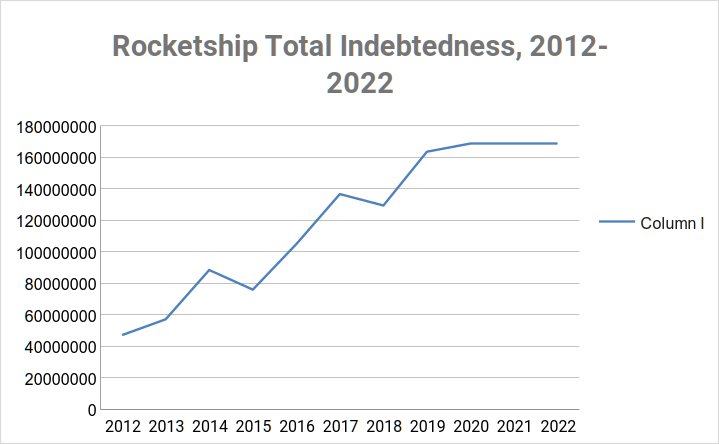
\includegraphics[width=\textwidth,keepaspectratio]{Debt}%
%   \caption{Rocketship Indebtedness, 2012-2022}%
%   \label{fig:total_debt}
% \end{figure}

% \begin{figure}[ht]
%   \centering
%   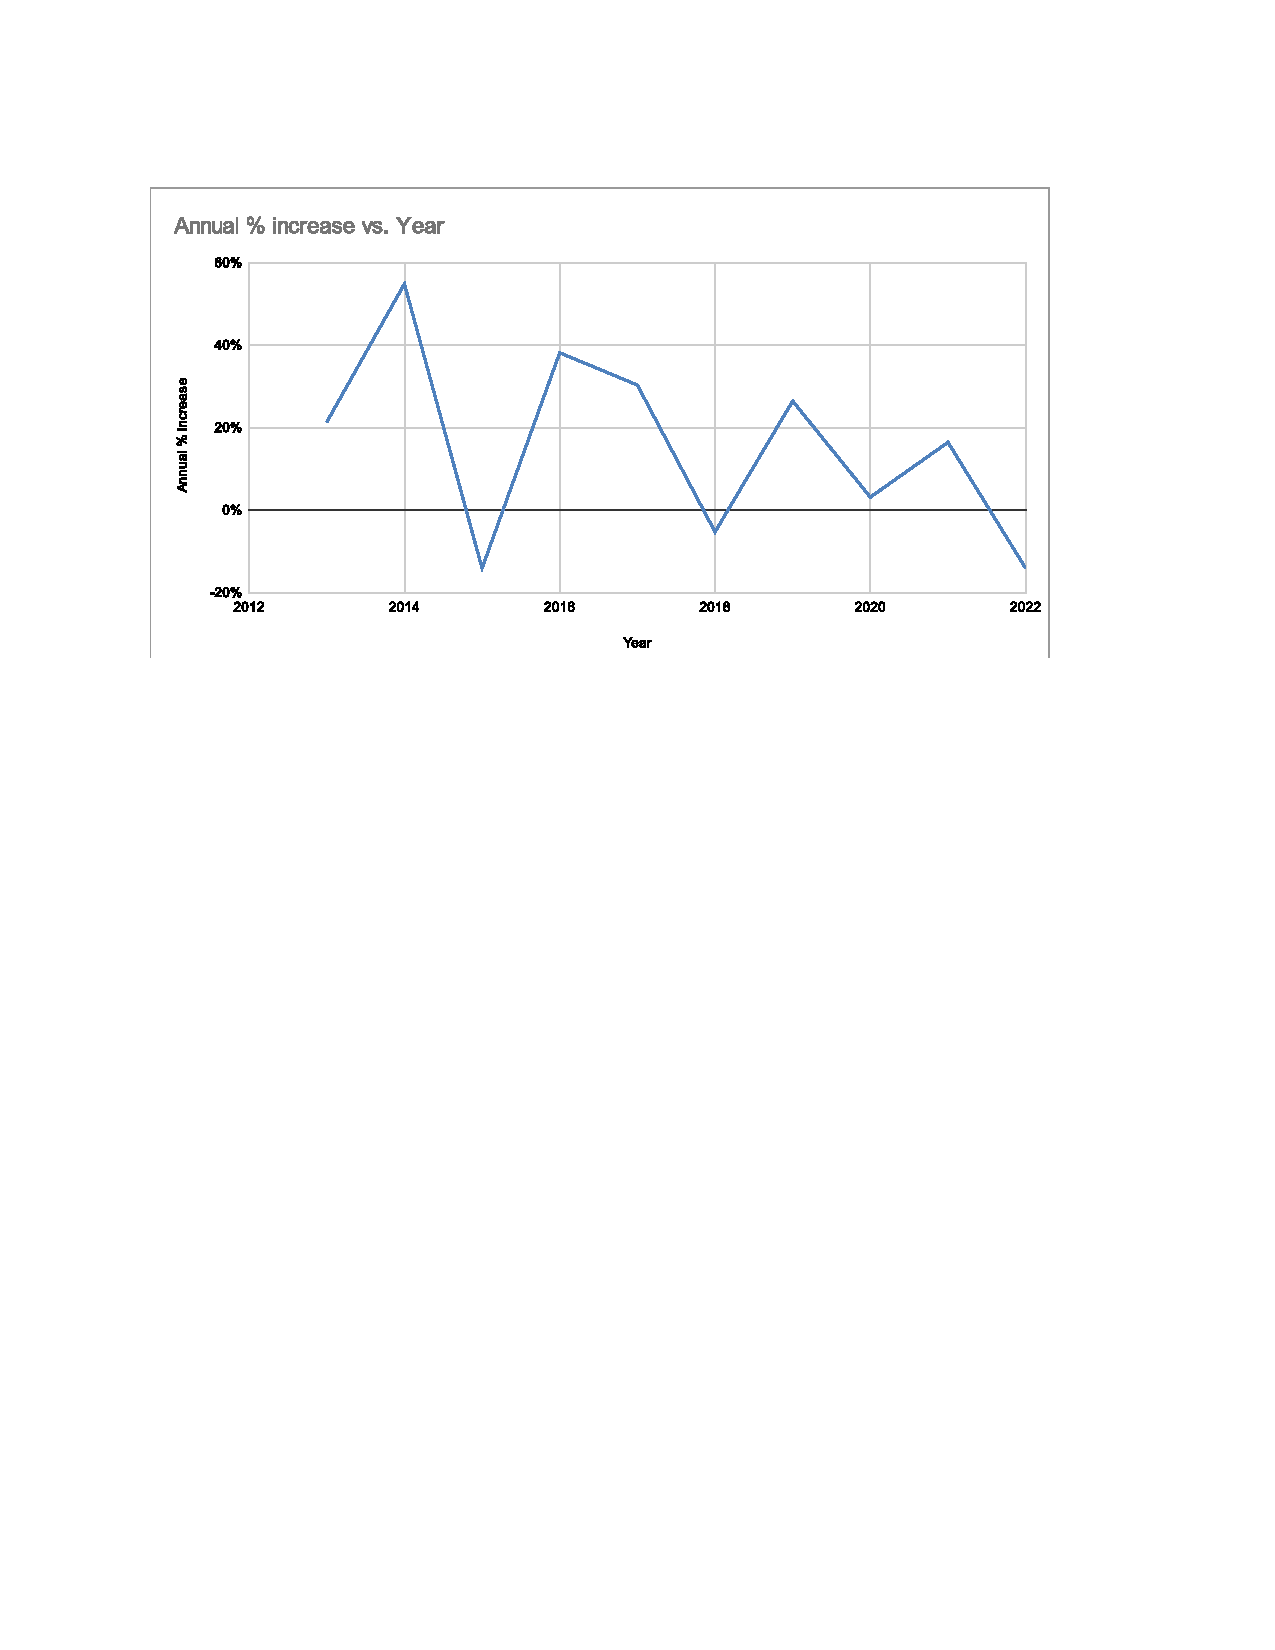
\includegraphics[width=\textwidth,keepaspectratio]{Annual_Debt_Increases}%
%   \caption{Rocketship Indebtedness, 2012-2022}%
%   \label{fig:annual_debt_increases}
% \end{figure}

\subsubsection{Financing Debt}\indent%
\label{sec:financing_debt}

\paragraph{Letters of Credit}
\paragraph{Municipal Bonds}
\paragraph{Conduit Bonds}

\subsection{Non-Debt Financing}\indent%
\label{sec:non_debt_financing}

\subsubsection{Donations and Grants}\indent%
\label{sec:donations_grants}

\subsubsection{Forgiveness of Debt}\indent%
\label{sec:forgiveness_debt}

\subsubsection{Loans}\indent%
\label{sec:loans}

\subsubsection{Venture Funds}\indent%
\label{sec:venture_funds}

\subsection{The New Markets Tax Credit}\indent%
\label{sec:NMTC}

The New Markets Tax (NMTC)credit of 39\% (5\% for the first 3 years, and 6\% for the remaining 4 years) can be applied to federal income taxes due. Since there is a compounding effect, the nominal 39\% is actually worth over 41\% of the initial investment. Note that the investments which generate a tax due likely themselves have a return. With these kinds of incentives, it's no wonder that the New Markets Tax Credit is popular. But one should not be deceived into thinking that just because New Markets Tax Credits must be made in economically depressed area that investors are investing out of the goodness of their heart. The tax credit investment is nearly without risk because the tax credit is guaranteed as long as the charter school remains open. If the school stays open for seven years, the risk is zero (unless the federal government shuts down).

An example will help make it clear how the NMTC works. Suppose I am a high wealth individual with a marginal tax rate of 37\% (the highest bracket), and suppose my investments return 10\% per annum.
\begin{quotation}\OnehalfSpacing%
  \noindent{}(All dollar amounts are in thousands) \\
  \noindent{}Given \$2,351 to invest \\
  \noindent{}Divided into a \$1,000 qualified NMTC investment and \$1,351 in some other investment. \\
  \noindent{}In the NMTC case, we have \$1,000 $\times$ 10\% return $\times$ 37\% income tax = \$37 tax due on \$100 profit, which means we get back \$1,000 + (\$1,000 $\times$ 0.1) - (\$1,000 $\times$ 0.37) = \$1,063 after taxes, in addition to a \$50 tax credit. \\
  
  \noindent{}In the non-qualifying investment, we have \$1,351 $\times$ 10\% return $\times$ 37\% income tax = \$50 tax due, which is exactly equal to the tax credit in the NMTC case.\\
  \noindent{}But we also have the return on the investment whose tax due was equal to the NMTC tax credit: \$,1351 + (\$1,352 $\times$ 0.1) = \$1,486.\\
  \noindent{}Combined, we get back \$1,063 + \$1,486 = \$2,549 for a 8.4\% net return after taxes, with effectively no risk.
  \\
  In general, the after tax return of an investment with a pre-tax return of 10\% for a high wealth individual is 6.3\%, so the NMTC after tax return is 33.3\% higher with almost no risk.
\end{quotation}

\subsubsection{Location and Concentration Grants}\indent%
\label{sec:location-concentration-grants}

\subsubsection{Student Instruction and Support}\indent%
\label{student_instruction_support}

\section{Gaps,  Anomalies, and Discrepancies}\indent%
\label{sec:gaps_anomolies_discrepencies}

This section is concerned with what wasn't found during our investigation. Gaps would be where data was expected, but none was found. Anomalies are where data was found, but it differed from what was expected, and discrepancies are where data was found but conflicted with other data which was found.

In an enterprise as large as Rocketship is now (\$190M+ budget), there are bound to be unintentional gaps, anomalies, and discrepancies without any implication of nefarious purposes. Further, as Berman and Knight emphasize, accounting involves making assumptions, estimates, and judgment calls; it is not an exact science.
\begin{quotation}
  The art of accounting and finance is the art of using limited data to come as close as possible to an accurate description of how well a company is performing.
  \sourceatright{\parencite[4-5]{Berman.Knight2013}}
\end{quotation}

So, the mere existence of gaps, anomalies, and discrepancies is not an indication of fraud. Fraud is deliberate, but gaps, anomalies, and discrepancies can occur because of differing assumption, simple oversight, or (unfortunately) plain incompetence.

%****************************************
%**** Gaps ******************************
%****************************************
\subsection{Gaps}\indent%
\label{sec:gaps}
\begin{itemize}
  \item IRS Form 990 for the tax year 2015–2016 cannot be found by looking in the locations where the other Form 990s were found.
  \begin{itemize}
    \item the IRS web site
    \item the Rocketship web site
    \item web sites belonging to organizations which specialize in tracking the finances of non-profits
  \end{itemize}
\end{itemize}

%****************************************
%**** Anomalies *************************
%****************************************
\subsection{Anomalies}\indent%
\label{sec:anomalies}
\begin{itemize}
  \item It appears that the Rocketship Business Committee only reviews and approves already signed checks in excess of \$100,000. Two things are anomalous here:
  \begin{enumerate}
    \item Rather than reviewing and approving purchase orders (i.e. before signature), the Rocketship Business Committee only retroactively approves checks (after signature). It is not known if those checks have already been sent to their respective payees.
    \item Rather than approving checks for any amount, only those above \$100,000 are reviewed and approved.
  \end{enumerate}
  \item The audited financial statements use a level of materiality that is three times higher than that used by a public school district (LASD) whose budget is half the size of Rocketship's, i.e. Rocketship's level of materiality is 50\% higher than expected..

  \item \textbf{Administrative Expenses vs Total Expenses}\\
  % Using functional expenses from the 2021-2022 school year as an example, Rocketship spent \$151,416,849 on educational programs, \$33,683,700 on program support, and \$46,401,574 on management and general expenses.  The management and geneal expenses thus are approx 30\% of what was spent on educational programs. In the Business Committee presentation, \textcite{Mukhopadhyay2013}, Rocketship says that the fees they charge individual schools are 35\% of revenue, consisting of a 20\% management fees and a 15\% facility fee. 

  Rocketship administrative expenses are considerably higher than what is allowed for public school districts. Using the statement of activities for the 2021-2022 school year as an example, Rocketship spent \$132,441,662 on educational programs and \$22,879,450 on administration.  Administrative expenses thus are approx 17\% of educational programs. (In a  Business Committee presentation, \textcite{Mukhopadhyay2013}, Rocketship says that the fees they charge individual schools are 35\% of revenue, consisting of a 20\% management fees and a 15\% facility fee.) This compares unfavorably with public school districts which are limited to 9\% of revenue for administrative expenses.

  If one counts fundraising as an administrative expense (\$507,147 in 2021–2022), then the anomaly is even more pronounced.
k  \item \textbf{Functional Expenses} This list of functional expenses that Rocketship has chosen to use differs from the list used in IRS Form 990, Part IX. This makes it nearly impossible to cross check (triangulate) data from Form 900 and the audited annual financial statements.
\end{itemize}

%****************************************
%**** Discrepencies *********************
%****************************************
\subsection{Discrepancies}\indent%
\label{sec:discrepancies}

The following discrepancies were found:
\begin{itemize}
  \item \textbf{Annual Financial Statements and Form 990s}\\
  The annual audited financial statements have several entries which also appear in the IRS Form 990, the federal tax return for organizations exempt from income tax, i.e. charities, religious organizations, private foundations, some political organizations, and other non-profits. For example, on June 30, 2015, the Consolidated Statement of Financial Position for 2014-2015 shows net assets to be \$10,562,747 (p.3) whereas the Form 990 (2014) show them to be \$13,968,882, a 32\% difference. Analysis of this discrepancy is limited and is insufficient to determine if the difference is the result of differing accounting practices or is a reflection of a more serious underlying problem.

  Similar discrepancies exist for functional expenses, among other categories.
  \item \textbf{Functional Expenses}\\
  \begin{itemize}
    \item \textbf{Accounting expenses}\\
    For the years ended 2019–2022, accounting expenses were \$166,059 in 2019, more than doubling to \$423,683 in 2020, roughly halving to \$264,784 in 2021, before more than tripling to \$848,221 in 2022. No mention is made of these substantial swings in accounting expenses in the \textit{Notes to Consolidated Financial Statements} for 2022.
    \item \textbf{Travel}\\
    In 2022, a total of \$2,635,011) was spent on travel which is over \$200,000 per month. This represents about 130 cross-country business class trips per month (at \$1700 per trip), or 440 economy class trips per month (at \$500 per trip). No explanation either for the need for this much travel or nor its cost was provided in the \textit{Notes to Consolidated Financial Statements}.
    \item \textbf{Salaries} For year 2018–2019, salaries are shown as \$54,294,263 on the audited statement of functional expenses. Yet, adding lines 5 (executive compensation), 7 (other salaries), 8 (pension plan), and 9 (other employee benefits) from Form 990 (2018–2019) yields \$54,516,782 which is close, but not quite the same as the amount shown in the audited statements. Further, it is not even clear that those lines and only those should sum to the same amount as ``Salaries'' in the audited statement of functional expenses.  For example, should pensions be counted as part of salaries? 
  \end{itemize}
\end{itemize}

\section{Issues of Equality and Equity}\indent%
\label{sec:issues_equality_equity}

Ostensibly, issues of equality and equity are at the heart of why Rocketship exists. Their vision is to ``eliminate the achievement gap in our lifetime.''(Our Mission \& Model. \url{https://www.rocketshipschools.org/about/mission-and-model})\footnote{Uncharitably, depending on whose lifetime Rocketship is referring to, the elimination of the achievement gap could be 30–60 years out. Included in this span of years is at least one pandemic, one major earthquake, several depressions or recessions, and numerous government shutdowns.} Their mission is to ``catalyze transformative change in low-income communities through a scalable and sustainable public school model that propels student achievement, develops exceptional educators, and partners with parents who enable high-quality public schools to thrive in their community.''(ibid.) These are laudable goals, but not unique to Rocketship or other charter schools.

Rocketship locates all of its schools in high poverty areas\footnote{areas where 20\% live in poverty or where the median family income less than 80\% of the area median family income\parencite[13-14]{CDFI2020}} where public schools are struggling to provide a quality education to all. Had they not done so, investors would not have been able to take advantage of the NMTC program. Despite being located in high poverty areas, Rocketship claims that its elementary schools are among the best in the nation. An argument can be made that all Rocketship can actually claim is that their students are among the best standardized test takers in the nation because there no evidence that Rocketship students continue their formal education (middle school, high school, college, university) do any better than public schools students (Nine Rocketship Schools Recognized as Among the Best in the Nation by US News \& World Report, \url{https://www.rocketshipschools.org/nine-rocketship-schools-recognized-as-among-the-best-in-the-nation-by-us-news-world-report/}). As previously mentioned, \textcite{Lubienski.Lubienski2014} have shown that the NAEP test results of public schools are higher than those of charter schools, all things considered. Of course this does not mean that Rocketship couldn't be an outlier whose students do better in the long run than those of other public or charter schools, but the only evidence that has been presented, like other CREDO publications, has not been well received.\footnote{Stanford University's CREDO (Center for Research on Education Outcomes) makes the case that ``from 2015 to 2019, the typical charter school student in our national sample had reading and math gains that outpaced their peers in the traditional public schools (TPS) they otherwise would have attended.'' \parencite{Raymond.etal2023}. However, this study has not been well received: ``A CREDO report compares charter school students’ learning in reading and math to students in traditional public schools. The report should be approached with caution by policymakers given the nonexperimental design that renders it unable to fully account for the factors that drive families to choose charter schools. In addition, the report presents its findings using an unconventional metric that makes it difficult to understand the policy implications, potentially misleading policymakers. The magnitude of the main findings fails to meet the minimum threshold experts consider to be a meaningful educational intervention.'' \parencite{Ferrare2023}}

%%% mode: latex
%%% TeX-master: "Rocketship_Education-An_Exploratory_Public_Policy_Case_Study"
%%% End: